% 2021年北京高考数学第4题解析图1：直角四面体
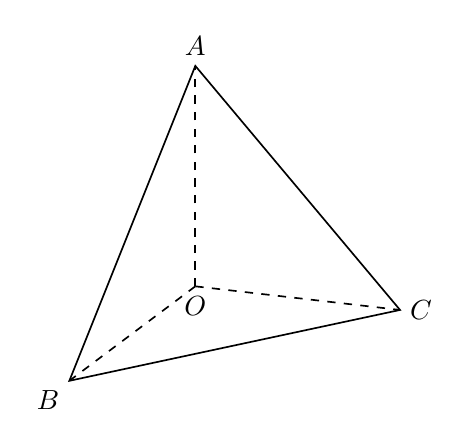
\begin{tikzpicture}[>=stealth,line width=0.6pt,font=\normalsize]
  \coordinate (O) at (0,0);
  \coordinate (A) at (0,2.8);
  \coordinate (B) at (-1.6,-1.2);
  \coordinate (C) at (2.6,-0.3);

  \draw[dashed] (O) -- (A);
  \draw[dashed] (O) -- (B);
  \draw[dashed] (O) -- (C);
  \draw (A) -- (B) -- (C) -- cycle;

  \node[below] at (O) {$O$};
  \node[above] at (A) {$A$};
  \node[below left] at (B) {$B$};
  \node[right] at (C) {$C$};
\end{tikzpicture}
